\documentclass[11pt]{article}


\title{Federated Truth Discovery for Mobile Crowdsensing with Privacy-Preserving Trustworthiness Assessment}

\author{Leye Wang$^{1,2}$, Guanghong Fan$^{1,2}$, Xiao Han$^{3,}$\footnote{Corresponding author} \\
 \small $^1$Key Lab of High Confidence Software Technologies (Peking University), Ministry of Education, China \\
\small$^2$School of Computer Science, Peking University, China\\
\small$^3$School of Information Management and Engineering, Shanghai University of Finance and Economics, China\\
\texttt{\small leyewang@pku.edu.cn, fgh@stu.pku.edu.cn, xiaohan@mail.shufe.edu.cn}
}

\begin{document}
	
\maketitle

\begin{abstract}
With the prevalence of smart mobile devices empowered by considerable sensing capabilities, crowdsensing has become one promising way to sense urban phenomena (e.g., traffic and environment) at a large scale. In crowdsensing, a fundamental issue is discovering the truth from participants' noisy sensed data. Traditionally, participants need to upload their raw sensed data with locations for truth discovery, but this may leak participants' private information such as home and work locations. In this paper, we propose a federated truth discovery method that can learn the truth without collecting participants' sensed data and locations. Our method ensures that the obtained truth quality has no performance loss compared to the original truth discovery method if all the participants keep online; even if some participants lose connections unpredictably, our method can still learn the truth based on rest participants' data.
Meanwhile, as participants' sensed data are unknown to the server, it is hard for the crowdsensing organizer to justify each participant's sensing trustworthiness. This brings difficulties to crowdsensing management such as participant recruitment and incentive allocation. We further propose a federated ranking mechanism to generate a leader-board for participants' trustworthiness, which can also tolerate participants' connection loss. Both theoretical analysis and real-data empirical evaluations have been done to verify the effectiveness of FedTruthFinder.

\end{abstract}

\section{Introduction}

With the popularity of smart mobile devices, such as smartphones, pads, and vehicles, crowdsensing has become one promising paradigm for sensing urban dynamics \cite{Leye-ganti2011mobile}. A typical crowdsensing process first recruits participants and then asks them to upload the data of interest to the central server. Afterward, the server aggregates the data from participants toward a synthetic sensed result \cite{Leye-zhang20144w1h,Leye-ma2014opportunities}. While each participant's sensed data may include noise, an important issue is how to ensure the accuracy of the aggregated sensed result, often called \textit{truth discovery} \cite{Leye-wang2012truth,Leye-meng2015truth,Leye-Wang2014SurrogateMS}.

Many research studies have been devoted to the truth discovery for crowdsensing applications. Generally, most relevant studies model participant trustworthiness and sensed data confidence iteratively to obtain the final aggregated sensed result \cite{Leye-yin2008truth}. The basic idea is that a high-credit participant's sensed data should be assigned with high confidence; a user whose sensed data are more confident should be more trustworthy. While this has been verified to be effective, the iterative computation process needs a central server to collect every participant's raw sensed data, which may bring privacy threats to crowdsensing participants. For example, crowdsensing usually asks participants to do sensing tasks at specific locations, and thus most sensed data are associated with detailed location information \cite{Leye-zhang20144w1h}. The traditional truth discovery process would inevitably leak crowdsensing participants' visited locations during sensing periods, which may be exploited by malicious third parties to conduct serious location privacy breaches such as physical stalking \cite{Leye-Primault2019TheLR}. With the user privacy and personal data regularization (e.g., General Data Protection Regulation\footnote{\url{https://gdpr.eu/eu-gdpr-personal-data}}) becoming more and more important nowadays, we believe that a privacy-preserving truth discovery algorithm is urgently required for facilitating more extensive crowdsensing campaigns in practice.

Privacy-preserving truth discovery has been recently studied in crowdsensing.  Existing studies are usually based on some hardly realized assumptions such as every participant being always online and/or non-colluding \cite{Leye-Miao2015CloudEnabledPT,Leye-Miao2017ALP,Leye-Miao2019PrivacyPreservingTD}\footnote{Some participants' relations can be very close such as family members, and thus it is non-reasonable to assume that they will not collude with each other.}, or two non-colluding servers (or fog nodes) are required \cite{Leye-Tang2018NonInteractivePT,Leye-Zheng2018LearningTT,Leye-Zhang2021ReliableAP,Leye-ZHANG2020101848}. These assumptions hinder the practical applications of the prior mechanisms.
More importantly, almost all the prior studies do not discuss two fundamental issues in privacy-preserving truth discovery.

i) \textbf{Participants' Completed Tasks Protection.} Existing mechanisms focus on protecting participants' sensed data, but most assume that participants' completed tasks are known to the crowdsensing server \cite{Leye-Xu2019EfficientAP,Leye-Miao2015CloudEnabledPT,Leye-Miao2019PrivacyPreservingTD,Leye-Zheng2018LearningTT}. However, sometimes task information is more sensitive than sensed data. Suppose the tasks are air quality sensing at certain points of interest. If a participant's task completion information is disclosed (e.g., finish a sensing task at the Times Square NYC), then her location is revealed without the need to know her sensed air quality value.

ii)  \textbf{Participants' Trustworthiness Assessment.} Trustworthiness assessment is a key part of crowdsensing for participant recruitment and incentive design \cite{Leye-Peng2018DataQG}, while privacy-preserving truth discovery needs to hide participants' trustworthiness scores for privacy protection. To address the dilemma, a privacy-preserving trustworthiness assessment method needs to be proposed.

In this paper, we aim to design a novel and practical privacy-preserving truth discovery mechanism for crowdsensing to overcome the pitfalls of prior studies. In particular, our design follows the federated learning (FL) paradigm \cite{Leye-konevcny2016federated,Leye-yang2019federated}. We thus call our method as \textit{FedTruthFinder}. In general, FL requires user clients to do some local computation (e.g., learning the gradients for updating the parameters of the model) on their devices and then only upload the computation results instead of raw data. For a specific algorithm, the local computation and uploading process usually incorporates certain secure mechanisms (e.g., homomorphic encryption and secure multi-party computation) to ensure that no user privacy is leaked theoretically \cite{Leye-chai2020secure,Leye-liu2020secure}.
Based on FL, we aim to consider the following specific issues in the design of FedTruthFinder.


\textbf{No Accuracy Loss}: We expect that FedTruthFinder will not hurt the accuracy of the aggregated sensed results compared to the centralized truth discovery. Without the loss of accuracy, crowdsensing organizers would be likely to adopt the method in practice.

\textbf{No Third Party}: Crowdsensing involves a central server and a set of participants' clients. To make FedTruthFinder easy to deploy, we do not want to introduce any more third parties which are usually hard to find in reality \cite{Leye-Bonawitz2017PracticalSA,Leye-Wang2017LocationPT}.


\textbf{Robustness against Unpredictable Connection Loss}: While crowdsensing participants travel around the whole city, their device connection with the central server is not always stable. Hence, it is necessary to make FedTruthFinder effective when some participants lose connections suddenly.



With the above issues in consideration, this paper makes the following contributions:

(1) To the best of our knowledge, this paper is the first study that addresses the problem of privacy-preserving crowdsensing truth discovery with (i) \textit{participants' completed task protection}, and (ii) \textit{participants' trustworthiness assessment}.

(2) We propose \textit{FedTruthFinder}, a novel privacy-preserving truth discovery mechanism following the federated learning paradigm \cite{Leye-yang2019federated}. FedTruthFinder does not need any third party and can tolerate participants' unpredictable connection loss. The two key components of FedTruthFinder are (i) \textit{federated confidence computation} to learn the probability of a sensed event, and (ii) \textit{federated trustworthiness ranking} to assess participants' sensed data quality.

(3) We have conducted both theoretical analysis and empirical evaluations for FedTruthFinder. In particular, FedTruthFinder can reduce the system failure probability significantly compared to state-of-the-art privacy-preserving truth discovery approaches~\cite{Leye-Bonawitz2017PracticalSA,Leye-Xu2019EfficientAP}, and achieve good detection accuracy.


\section{Preliminary: Truth Discovery}
\label{sec:preliminary}

\begin{figure}
	\centering
	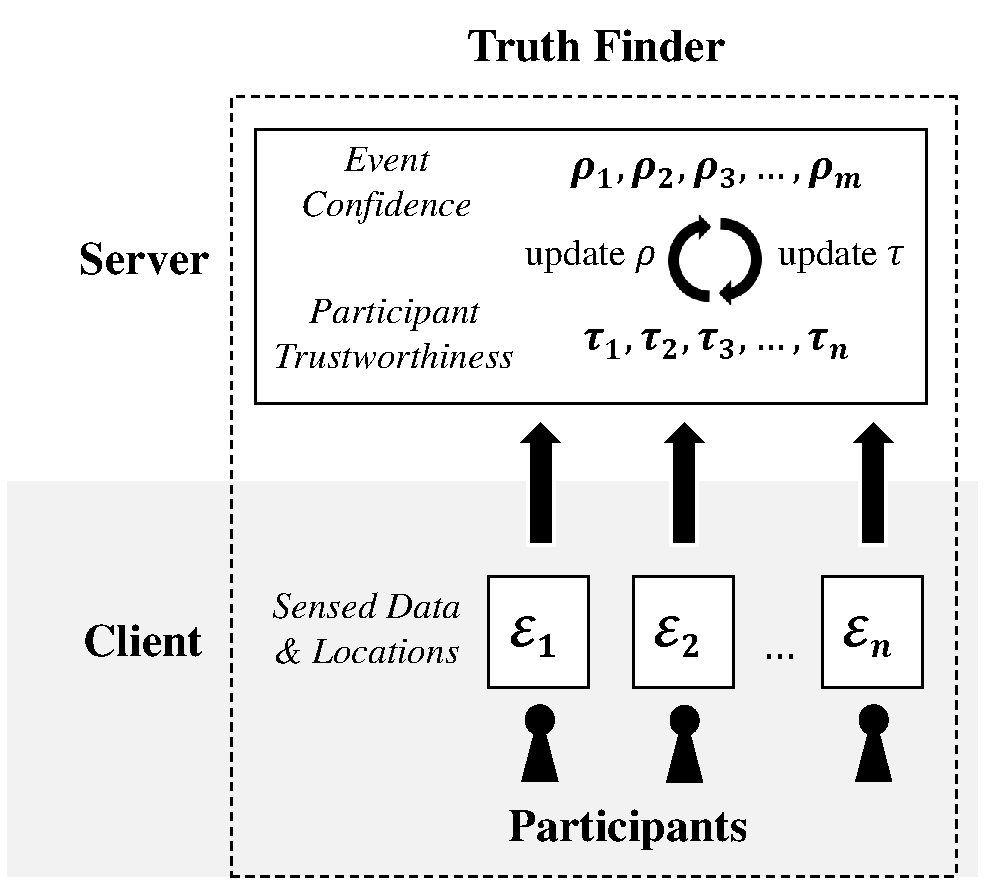
\includegraphics[width=.5\linewidth]{submissions/LeyeWang/fig/truthfinder.pdf}
	\caption{Overview of Iterative Truth Discovery}
	\label{fig:truthfinder}
	\vspace{-1em}
\end{figure}


Truth discovery algorithms usually follow an iterative method to calibrate user trustworthiness and data confidence alternatively until convergence \cite{Leye-yin2008truth}. Figure~\ref{fig:truthfinder} shows the framework of iterative truth discovery methods. In this paper, for clarity, we assume that sensed data is a binary spatial event. That is, for a specific location, the sensed data can be 1 or 0. Our method can be easily extended to multi-class and continuous-value events (see Appendix).

As shown in Figure~\ref{fig:truthfinder}, first, participants upload all of their sensed data and locations $\mathcal E_i$  to the central server. The central server would assign an initial trustworthiness score $\tau_i$ to each participant $u_i$ (e.g., 0.9 by assuming that 90\% of the sensed data are accurate). Then, for each sensed event $e_j$, the truth discovery algorithm will calculate its confidence $\rho_j$ (i.e., the probability of $e_j = 1$) by considering the users who have sensed $e_j$ as:
\begin{equation}
\rho_j = F_\rho(\mathcal U_{j,1}, \mathcal U_{j,0})
\label{eq:event_confidence}
\end{equation}
where $\mathcal U_{j,k}$ is the users who have sensed the event $e_j$ with the reported data $k$; $F_\rho$ is an event confidence calculation function which we will elaborate on later.

With $\rho_j$ for each event $e_j$, we can then update the trustworthiness score $\tau_i$ of each participant $u_i$ by:
\begin{equation}
\tau_i = F_\tau(\mathcal E_{i,1}, \mathcal E_{i,0})
\end{equation}
where $\mathcal E_{i,k}$ is the users' sensed event set with the reported data $k$; $F_\tau$ is a user trustworthiness calculation function which we will elaborate on later.

Once $\tau_i$ is updated for each user $u_i$, we can continue updating $\rho_j$ for each event $e_j$ according to Eq.~\ref{eq:event_confidence}, and so on, leading to an alternative updating process for both $\tau_i$ and $\rho_j$. This process can be terminated after a fixed number of iterations or until convergence. Next, we elaborate on the common choices of $F_\rho$ and $F_\tau$ in literature.

\textbf{Sum Function}

An intuitive selection of the updating functions of $F_\rho$ and $F_\tau$ is the weighted sum:
\begin{equation}
\rho_j = F_\rho(\mathcal U_{j,1}, \mathcal U_{j,0}) = \frac{\sum_{u_i \in \mathcal U_{j,1}} \tau_i}{\sum_{u_i \in \mathcal U_{j,1}} \tau_i + \sum_{u_k \in \mathcal U_{j,0}} \tau_k}
\label{eq:rho_function_sum}
\end{equation}
\begin{equation}
\tau_i = F_\tau(\mathcal E_{i,1}, \mathcal E_{i,0}) = \frac{\sum_{e_j \in \mathcal E_{i,1}} \rho_j + \sum_{e_k \in \mathcal E_{i,0}} 1-\rho_k}{|\mathcal E_{i,1}|+|\mathcal E_{i,0}|}
\label{eq:tau_function}
\end{equation}

\textbf{Logistic Function}

Another widely used updating function is the Logistic function \cite{Leye-yin2008truth}. Its basic idea is seeing every user independently, so that the probability of event happening, i.e., $e_j=1$, can be formulated as:
\begin{equation}
	\rho_j = 1 - \prod_{u_i \in \mathcal U_{j,1}} (1-\tau_i)
\end{equation}
As $1-\tau_i$ may often be small and multiplying many of them may lead to underflow, prior studies proposed to use the logarithm to define a log-trustworthiness score of $u_i$ as \cite{Leye-yin2008truth}:
\begin{equation}
	\tau_i^* = - \ln(1-\tau_i)
\end{equation}
Similarly, a log-confidence score of event $e_j$ is defined as:
\begin{equation}
	\rho_j^* = - \ln(1-\rho_i)
\end{equation}
Then, we can infer
\begin{equation}
	\rho_j^* = \sum_{u_i \in \mathcal U_{j,1}} \tau_i^*
\end{equation}
The above equation does not consider the users' trustworthiness who report $e_j=0$, and thus we refine it:
\begin{equation}
	\rho_j^* = \sum_{u_i \in \mathcal U_{j,1}} \tau_i^* - \sum_{u_k \in \mathcal U_{j,0}} \tau_k^*
\end{equation}
Finally, a logistic function is used to calculate the final confidence $\rho_j$ of event $e_j$ \cite{Leye-yin2008truth}:
\begin{equation}
	\rho_j = F_\rho(\mathcal U_{j,1}, \mathcal U_{j,0}) = (1+e^{-\rho_j^*})^{-1}
	\label{eq:rho_function_log}
\end{equation}
$\tau_i$ is updated same as Eq.~\ref{eq:tau_function}. 


\section{Federated Truth Discovery: Overview and Key Issues}

\subsection{Overall Design}

\begin{figure}
	\centering
	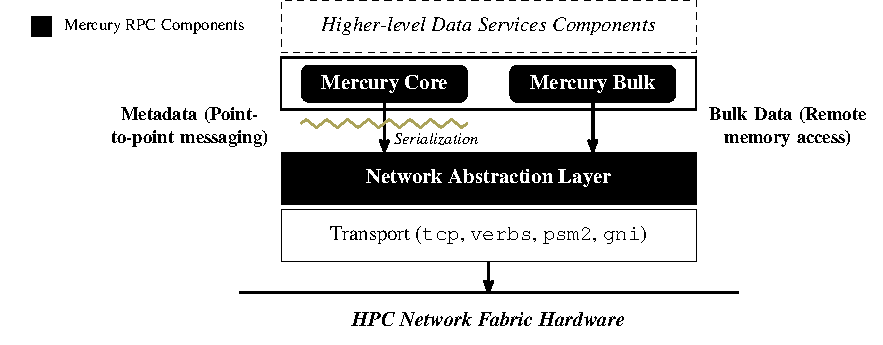
\includegraphics[width=.8\linewidth]{submissions/LeyeWang/fig/overview.pdf}
	\caption{Overview of FedTruthFinder}
	\label{fig:overview}
\end{figure}

Figure~\ref{fig:overview} overviews the workflow of our method \textit{FedTruthFinder}. The general design principle follows the federated learning paradigm \cite{Leye-yang2019federated}, which requires the user clients to conduct local computations of their raw data and then upload processed data that do not reveal the user's privacy to the server. With these uploaded privacy-preserving data, the server can still find the aggregate truth of the sensed events, the same as the server receiving the raw sensed data and locations from participants.

By analyzing the original truth discovery algorithm in the previous section, we note that there exist two alternative computation processes: (i) \textit{$\rho$-computation}: updating the confidence $\rho_j$ for each event $e_j$, and (ii) \textit{$\tau$-computation}: updating the trustworthiness $\tau_i$ for each participant $u_i$. In the two computation processes, $\tau$-computation (e.g., Eq.~\ref{eq:tau_function}) can be naturally offloaded to each participant $u_i$'s device, as long as the server sends all the current $\rho_j, \forall e_j$ to the participants. However, $\rho$-computation needs to know each user's sensed data (and locations) and then do aggregation (e.g., sum). This needs a dedicated design to enable the privacy-preserving truth discovery, which will be illustrated in Sec.~\ref{sec:truth_computation}.

Besides, the trustworthiness of each participant's sensed data (i.e., $\tau_i$) is a key metric in crowdsensing organization for participant recruitment and incentive allocation. Hence, we also design a federated privacy-preserving mechanism to rank participants' trustworthiness. Particularly, instead of transferring raw $\tau_i$ to the server, we leverage certain security mechanisms to upload $f(\tau_i)$ to the server, while $f(\tau_i)$ keeps the same ranking orders as $\tau_i$. Particularly, in FedTruthFinder, $f(\tau_i)=r_1\tau_i+r_2\tau_i^2+...+r_k\tau_i^k$, where $r_i>0$.  In this regard, even though the server cannot know the specific $\tau_i$ of each participant $u_i$, the ranked list of participants according to the trustworthiness can still be learned with $f(\tau_i)$. Specifically, during the whole computation process, the server cannot know $r_i$, and each participant will also not know all the $r_i$, so that none of the server or participant can infer other participants' private $\tau_i$. How to compute $f(\tau_i)$ securely will be introduced in Sec.~\ref{sec:trust_ranking}.

\subsection{Key Issues}

\textbf{Issue 1. Privacy-Preserving $\rho$-computation}: \textit{Suppose there are a set of crowdsensing participants $\mathcal U$ and a set of spatial events to sense $\mathcal E$, each participant $u_i (\in \mathcal U)$ with sensed events $\mathcal E_{i,1} (\subseteq \mathcal E)$ and $\mathcal E_{i,0} (\subseteq \mathcal E)$ corresponding to the sensed value being $1$ and $0$, respectively. How to calculate confidence $\rho_j$ for each event $e_j (\in \mathcal E)$ while every participant $u_i$ will not leak $\mathcal E_{i,1}$, $\mathcal E_{i,0}$, and $\mathcal E_{i,1} \cup \mathcal E_{i,0}$ to the server and other participants?}

Some factors need to be carefully considered:

(1) \textbf{Computation}: In $\rho$-computation, the value to share is a complicated equation instead of a single value, and the equation may even be varied depending on the truth discovery algorithm implementation (e.g., Eq.~\ref{eq:rho_function_sum} or Eq.~\ref{eq:rho_function_log}).

(2) \textbf{Network Connection}: In crowdsensing, the network connections of mobile participants may not be always stable. Hence, our mechanism should tolerate the scenario when a few participants lose connections.

(3) \textbf{No Leakage of Task Completion}: For protecting participants' privacy, not only the sensed data but also the completed tasks (i.e., $\mathcal E_{i,1} \cup \mathcal E_{i,0}$) should not be disclosed.

\vspace{+.5em}
\noindent \textbf{Issue 2. Secure Trustworthiness Ranking}: \textit{Suppose there are a set of crowdsensing participants $\mathcal U$ and each participant $u_i (\in \mathcal U)$ has a private trustworthiness score $\tau_i$. How to rank participants according to $\tau_i$ while every participant $u_i$ will not leak $\tau_i$ to the server and other participants?}

Addressing this issue also needs to consider the unstable network connections of participant clients as aforementioned.


\textbf{Remark on security definition}: In this work, we assume that the crowdsensing server and participants are \textit{semi-honest (honest-but-curious)}: they will follow our designed protocol and not maliciously modify the inputs or outputs; however, the server and the participants will try their best to infer others' data from the data that they have received. Besides, our mechanism can defend against \textit{collusion attacks} to a certain extent (i.e., some participants may collude with each other), which we will elaborate on later.

\section{Federated Truth Computation}
\label{sec:truth_computation}

We first introduce a basic scheme for $\rho$-computation in a federated manner assuming no connection loss. Then, we improve the scheme to be against the participants' unpredictable connection loss. %Finally, we theoretically analyze the proposed algorithm.

\subsection{Basic Scheme of $\rho$-Computation with SSS}
\label{sub:basic_rho_computation}

In this section, we propose our basic scheme for the $\rho$-computation problem with the federated learning paradigm leveraging secret sharing. Given a spatial crowdsensing event $e_j$, we first consider $\rho$-computation with the sum function, i.e., Eq.~\ref{eq:rho_function_sum}.

\subsubsection{$\rho$-computation with the sum function.} Our process includes three steps as follows:


\textbf{Step 1 (Share Dispatching)}. Each participant $u_i$ dispatches $d_{ij}$ and $s_{ij}$ with secret sharing to all the $n$ participants ($\mathcal U = \{u_1\cdots u_n\}$), where
\begin{align}
	d_{ij} & =
	\begin{cases}
		\tau_i & \quad\quad e_j \in \mathcal E_{i,1} \\
		0 & \quad\quad e_j \in \mathcal E\setminus \mathcal E_{i,1}
	\end{cases}\\
	s_{ij} &=
	\begin{cases}
		\tau_i & \quad\quad e_j \in \mathcal E_{i,1}\cup \mathcal E_{i,0} \\
		0 & \quad\quad e_j \in \mathcal E\setminus(\mathcal E_{i,1}\cup \mathcal E_{i,0})
	\end{cases}
\end{align}
Specifically, $d_{ij}$ is divided into $n$ shares
$$\{d_{ij}^1,\cdots,d_{ij}^n\}$$
where $d_{ij}^1, \cdots, d_{ij}^{n-1}$ are random numbers and
$$d_{ij}^n = d_{ij} - \sum_{k=1}^{n-1} d_{ij}^k$$
Hence,
$\sum_{k=1}^n d_{ij}^k = d_{ij}$.
Then, $u_i$ sends $d_{ij}^k$ to $u_k$. Similarly, $s_{ij}$ is split to $n$ shares
$$\{s_{ij}^1,\cdots,s_{ij}^n=s_{ij}-\sum_{k=1}^{n-1} s_{ij}^k\}$$
and $u_k$ receives $s_{ij}^k$ from $u_i$.

\textbf{Step 2 (Client Summation)}. For each event $e_j$, an participant $u_k$ uploads $\hat d_{j}^k=\sum_{i=1}^n d_{ij}^k$ and $\hat s_{j}^k = \sum_{i=1}^n s_{ij}^k$ to the server.

\textbf{Step 3 (Server Aggregation)}. After receiving $\hat d_{j}^k$ and $\hat s_{j}^k$ from $\forall u_k \in \mathcal U$, the server can add them together:
\begin{align}
	d_j & = \sum_{k=1}^n \hat d_{j}^k = \sum_{k=1}^n\sum_{i=1}^n d_{ij}^k = \sum_{i=1}^n \sum_{k=1}^n d_{ij}^k = \sum_{i=1}^n d_{ij} \\
	s_j & = \sum_{k=1}^n \hat s_{j}^k = \sum_{k=1}^n\sum_{i=1}^n s_{ij}^k = \sum_{i=1}^n \sum_{k=1}^n s_{ij}^k = \sum_{i=1}^n s_{ij}
\end{align}
Then, $\rho_j$ is computed as:
\begin{equation}
	\rho_j = \frac{d_j}{s_j}
\end{equation}


\subsubsection{$\rho$-computation with the logistic function.} The computation process with the logistic function is not much different from the one with the summation function. Actually, for the event $e_j$, we only need to modify $d_{ij}$ to:
 \begin{align}
 	d_{ij} & =
 	\begin{cases}
 		-\ln(1-\tau_i) & e_j \in \mathcal E_{i,1} \\
 	    \ln (1-\tau_i) & e_j \in \mathcal E_{i,0}\\
 		0 & e_j \in \mathcal E\setminus(\mathcal E_{i,1}\cup \mathcal E_{i,0})
 	\end{cases}
 \end{align}
Besides, we do not need $s_{ij}$, so every participant $u_k$ only receives $d_{ij}^k$ from other $u_i \in \mathcal U$. Finally, in Step 3, we can compute $\rho_j$ as:
\begin{equation}
	\rho_j = (1+e^{-d_j})^{-1}
\end{equation}

\textbf{Remark on our novelty}. In our $\rho$-computation for an event $e_j$, the participant $u_i$ who has not sensed $e_j$ also needs to upload data to the server, e.g., $d_{ij}=s_{ij}=0$ for the sum function. As $d_{ij}$ and $s_{ij}$ are sent by secret shares, the other participants and the server would not know whether $u_i$ senses $e_j$ or not. In comparison, prior studies usually assume that participants send only the data of their sensed events, which may disclose user privacy from event information (e.g., event locations) \cite{Leye-Miao2015CloudEnabledPT,Leye-Miao2017ALP,Leye-Miao2019PrivacyPreservingTD,Leye-Zheng2018LearningTT,Leye-Zheng2020PrivacyAwareAE,Leye-Zhang2021ReliableAP}.

\subsection{Connection Robustness Improvement}

The basic scheme can learn $\rho_j$ in an ideal environment when all the participants are always online. In practice, participants move around and their network connections are often sporadic. This inspires us to make three improvements to the basic scheme design.

\subsubsection{Bias-avoidance adaptive truth updating.}
\label{sub:adaptive_truth_updating}
While participants may drop during the iterative truth discovery process due to bad connections, the original event confidence updating function would be ineffective. Specifically, if $u_i$ loses the connection at the $k^{th}$ iteration, $u_i$'s data would not be considered in the $\rho$-computation (e.g., Eq.~\ref{eq:rho_function_sum}) from then on. This leads to unreliable $\rho_j$ as the finally alive participants dominate the results. To address this pitfall, we propose an adaptive updating function for $k^{th}$ iteration's $\rho_{j,k}$ as,
\begin{equation}
	\rho_{j,k} = w_k F_\rho + (1-w_k) \rho_{j,k-1}
	\label{eq:rho_adaptive_update}
\end{equation}
where $F_\rho$ is an original event confidence updating function (e.g., sum and logistic). With Eq.~\ref{eq:rho_adaptive_update}, the data contribution of the participants who drop at the $k^{th}$ iteration can still be kept (by $\rho_{j,k-1}$) to avoid the truth bias toward alive participants. $w_k$ can be set as,
\begin{equation}
	w_k = (\frac{|\mathcal U_{alive,k}|}{|\mathcal U|})^\alpha
	\label{eq:adaptive_weight}
\end{equation}
where $\mathcal U_{alive,k}$ is the alive participants at the $k^{th}$ iteration. When alive participants decrease with more iterations, $w_k$ becomes smaller, reflecting that fewer participants should occupy lower weights. From our experiments, we find that $\alpha=3$ is a proper setting.

\subsubsection{Server-coordinated communication structure.}
\label{subsub:server_coordination}

In Sec.~\ref{sub:basic_rho_computation}, we assume that one participant $u_i$ can establish a secure communication channel with every other participant $u_k$ so as to transfer the secret share $d_{ij}^k$ and $s_{ij}^k$. Hence, each participant needs to establish $n-1$ channels with others. Considering the sporadic property of the mobile connections, this may not be easy for a participant to keep so many channels stable in practice. To alleviate this issue, we convert the peer-to-peer communication structure to a server-coordinated one. In the server-coordinated structure, every participant first transmits all the data to the server, and then the server dispatches the desired data to the corresponding participant. In this way, each participant  needs to establish \textit{only one} secure channel to the server.

To ensure that the transmitted data will not be directly observed by the server, we leverage a public-key encryption system to encrypt the data before the transmission. In particular, each participant $u_i$ first generates a pair of keys, the public key $pk_i$ and the private key $sk_i$. The public key $pk_i$ is sent to all the other participants (e.g., through the server) at the beginning of the crowdsensing campaign. For details, readers can refer to \cite{Leye-Bonawitz2017PracticalSA}.

Then, for computing $\rho_j$, each participant $u_i$ first transmits $E_i = \{\textit{Encrypt}(d_{ij}^k, pk_k)| k = 1\cdots n\}$ to the server.\footnote{If $s_{ij}$ is needed (e.g., for the sum function), it can be encoded in $E_i$ same as $d_{ij}$.} After receiving $n$ participants' $E_i$, the server re-organizes the received data and sends $\hat E_k = \{\textit{Encrypt}(d_{ij}^k, pk_k)| i = 1\cdots n\}$ to each participant $u_k$. Afterward, $u_k$ decrypts the received data with her private key, obtains $\{d_{ij}^k| i = 1 \cdots n\}$, and then uploads $\hat d_j^k = \sum_i d_{ij}^k$ to the server. The server can then recover $d_j = \sum_i d_{ij}$ from participants' uploaded  $\hat d_j^k$ and computes $\rho_j$ accordingly.

\subsubsection{$(t,n)$-Shamir secret sharing (SSS)} While the server-coordinated communication structure reduces the burden of secure channel establishing for mobile participants. It may still fail if a user loses the connection during the campaign and cannot link back. For example, suppose a participant $u_i$ has sent $E_i$ to the server and then quit the crowdsensing campaign (e.g., $u_i$'s mobile device runs out of battery). Then, in Step 3, the server will not be able to receive $\hat d_j^i$ from $u_i$, and thus cannot recover $d_j$.

To address this pitfall, in practical deployment, we can leverage the threshold secret sharing method proposed by Shamir \cite{Leye-shamir1979share}, namely \textit{$(t,n)$-Shamir secret sharing (SSS)}. With $(t,n)$-SSS, the server only needs to receive $t\ (t\le n)$ participants' $\hat d_j^i$ for recovering $d_j$. In particular, to leverage $(t,n)$-SSS to dispatch $d_{ij}$, we first create a $(t-1)$-polynomial:
\begin{equation}
	D_{ij}(x) = d_{ij}+a_{ij1}x+a_{ij2}x^2+\cdots+a_{ijt-1}x^{t-1}
\end{equation}
where $a_{ij1},\cdots, a_{ijt-1}$ are random numbers selected by $u_i$. Then, $u_i$ dispatches $D_{ij}(k)$ to $u_k$. If we obtain more than $t$ participants' $D_{ij}(k)$, according to linear algebra, we can infer $d_{ij}$.

Similar to Step 2 of our basic scheme, $\hat d_j^k = \sum_{i} D_{ij}(k)$ is uploaded to the server by each $u_k$. Then, in Step 3, after receiving more than $t$ participants' $\hat d_j^k$, the server will be able to infer $d_j = \sum_{i} d_{ij}$ according to the \textit{additive homomorphism property} of SSS \cite{Leye-shamir1979share}.

\textbf{Remark on our novelty}. In the truth discovery part, the key advantage of our mechanism beyond literature is its robustness against connection loss. Preliminary privacy-preserving truth discovery papers rarely consider the connection loss issue \cite{Leye-Miao2017ALP}. Some work tries to deal with drop-out users by letting alive participants send extra information \cite{Leye-Zhang2021ReliableAP,Leye-Wang2021AST}; however, when the connection condition is so bad that certain alive participants again lose connections during the extra information communication, this process would be uncontrolled and time-consuming. Recent work also adopts SSS to enhance connection robustness \cite{Leye-Xu2019EfficientAP}. The basic idea is using the double-masking secure aggregation algorithms proposed by \cite{Leye-Bonawitz2017PracticalSA}, and every participant needs \textit{two} connections to do event confidence computation for one iteration. In comparison, our mechanism only needs every participant to connect \textit{once} for one iteration of computation. Our numerical experiments (Sec.~\ref{sec:numeric_analysis}) will show that this connection reduction can lead to a significantly difference in the algorithm success probability (e.g., increasing the success probability from $1\%$ to $99\%$ under certain conditions).


\subsection{Theoretical Analysis}
\label{sub:theoretical_analysis_1}


\subsubsection{Correctness} The process to calculate $\rho_i$ in FedTruthFinder follows the original algorithm shown in Sec.~\ref{sec:preliminary}. Hence, we can obtain the same aggregate truth results as the original algorithm, as long as the SSS scheme is valid. In this regard, the correctness of our algorithm is theoretically guaranteed.


\subsubsection{Robustness to Connection Loss \& Security}
Setting $t$ to a small value allows our mechanism to tolerate more users dropping the campaign due to connection losses. Meanwhile, a small $t$ reduces the security level of our mechanism --- if $t$ participants collude with each other, they can recover the other participants' sensed data and locations, leading to privacy leakage.

\textbf{Theorem 4.1}. If there are $\le n-t$ participants losing the connection in one iteration of $\rho$-computation, the server can learn the event confidence $\rho_j$.

\textbf{Theorem 4.2}. If $t' (<t)$ semi-honest users collude with each other, they cannot infer any other users' secret information.

The two theorems hold based on the property of $(t, n)$-SSS.

\subsubsection{Complexity}
We analyze the algorithm from both communication and computation complexity perspectives. Particularly, since the participant clients are more sensitive to the communication and computation overhead, our current analysis focuses on the client side, while the server part analysis is similar.

\textbf{Communication Complexity - $O(nn_e)$}. For each participant client, she needs to transfer $n$ share pieces of the secret to the other participants and receive the corresponding shares from every other participant, so the complexity is $O(n)$ for one event. Suppose there are $n_e$ events, the total communication complexity is $O(nn_e)$.

\textbf{Computation Complexity - $O(nn_e)$}. Each client needs to do two local computation processes. The first process is to generate the random coefficients for $(t,n)$-SSS and calculate the secret shares sent to all the other participants (Step 1), which is $O(nn_e)$. The second process is to do local summation (Step 2), which is also $O(nn_e)$. Hence, the total computation complexity is $O(nn_e)$.


\section{Federated Trustworthiness Rank}
\label{sec:trust_ranking}

While FedTruthFinder learns the integrated event truth in a privacy-preserving manner, it brings a challenge in justifying participants' trustworthiness. For example, to incentivize the crowdsensing participants, it is a common strategy to pay the high-trustworthy participants (i.e., high-quality sensing results) with higher incentives. However, in FedTruthFinder, the sensing quality of each participant, i.e., the trustworthiness score $\tau_i$ is kept at each participant side and unknown to the server. Hence, how to assess participants' trustworthiness is required and challenging for FedTruthFinder.

In this section, we first illustrate a concrete case to describe that $\tau_i$ cannot be directly known to the server, otherwise the server may infer which event $u_i$ has sensed. As $\tau_i$ cannot be known to the server, we then design a secure ranking algorithm to let the server know every participant $u_i$'s ranking position of $\tau_i$ among all the participants without leaking $\tau_i$. Based on the ranked positions, the crowdsensing organizer can enable certain trustworthiness-aware incentive mechanisms, e.g., rewarding high-position participants with bonus, which can incentivize participants to compete with each other to get more high-quality sensed data \cite{Leye-Reddy2010ExaminingMF}.

\subsection{Privacy Leakage by Trustworthiness $\tau_i$}

Here, we illustrate an example to show the risk of revealing $\tau_i$ to the server for leaking participant $u_i$'s privacy.

Without the loss of generality, we assume that $u_1$'s $\tau_1 = 0.9$, and other $u_i$'s $\tau_i < 0.9\ (i\not=1)$. Suppose that one event $e_j$'s $\rho_j = 0.9$ after truth discovery, then we can easily infer that $u_1$ has sensed the event $e_j$ and the sensed result is $1$. This reveals the fact that $u_1$ has visited the location of $e_j$, leaking $u_1$'s location privacy.

Hence, participants cannot directly upload their $\tau_i$ to the server for incentive allocation. Next, we design a privacy-preserving method to enable trustworthiness-aware incentive allocation.

\subsection{Secure Trustworthiness Leader-board}

While revealing $\tau_i$ may leak participants' private information, we propose a secure ranking algorithm to learn a  leader-board regarding participants' trustworthiness for facilitating trustworthiness-aware incentive allocation.

Secure ranking algorithms have been studied for decades; however, prior studies cannot be directly applied in our scenario for two reasons. First, the communication overheads are usually high. Second, prior studies mostly assume that all the network connections are stable for all the parties, but this is unrealistic for crowdsensing.

Our secure ranking algorithm generally follows the design of \cite{Leye-tang2011secure}. However, the original design \cite{Leye-tang2011secure} cannot tolerate any participants to lose the network connections. We thus enhance it to ensure that the ranking algorithm can still work when certain participants lose connections.
The major steps of our federated trustworthiness leader-board generation mechanism are:

\textbf{Step 1}. First, we categorize all the participants into $(2t+1)$ groups, and thus each group includes $n/(2t+1)$ participants. We denote $gid(u)$ to refer to the group ID of participant $u$.

\textbf{Step 2}. For each user $u_i$, she shares $\tau_i$, $\tau_i^2$, ... , $\tau_i^{2t+1}$ with $(t+1, 2t+1)$-SSS to all the user groups. Specifically, a user $u_j$ will receive the share piece regarding $gid(u_j)$, denoted as $\tau_{i_1}(gid(u_j))$, $\tau_{i_2}(gid(u_j))$, ... $\tau_{i_{2t+1}}(gid(u_j))$ for $\tau_i$, $\tau_i^2$, ... , $\tau_i^{2t+1}$, respectively.

\textbf{Step 3}. For each user group $g_k$, it generates a random number $r_k (>0)$ and shares $r_k$ with $(t+1, 2t+1)$-SSS to all the user groups. That is, $u_j$ will receive $r_k$'s share regarding $gid(u_j)$, denoted as $r_k(gid(u_j))$.

\textbf{Step 4}. For each participant $u_j$, she calculates the following number with the $\tau_{i_k}(gid(u_j))$ received from $u_i$:
\begin{align}
h_{i}(gid(u_j)) &= \lambda(gid(u_j)) \sum_{k=1}^{2t+1} r_k(gid(u_j)) \tau_{i_k}(gid(u_j)) \\ &= \lambda(gid(u_j)) \gamma(gid(u_j))
\end{align}
where
\[
\left(\begin{array}{ccccc}
	1 &    1 & 1^2 & ...  & 1^{2t} \\
	1 &    2 & 2^2 & ... & 2^{2t}\\
	... & ... & ... & ...& ...\\
	1 & 2t+1 & (2t+1)^2 & ... & (2t+1)^{2t}\\
\end{array}\right)^{-1}
\]
\[
=\left(\begin{array}{ccccc}
	\lambda(1) &   \lambda(2) & \lambda(3) & ...  & \lambda(2t+1) \\
	... & ... & ... & ...& ...\\
	... & ... & ... & ...& ...\\
	... & ... & ... & ...& ...
\end{array}\right)
\]


\textbf{Step 5}. For each user group, we randomly select one participant $u_j$ to share $\{h_{i}(gid(u_j))| i \in [1,n]\}$ with $(t+1, n)$-SSS to all the $n$ participants. Each user $u_k$'s received shares from all the groups are denoted as $\{h_i(g, k)| i \in [1,n], g \in [1, 2t+1]\}$.

\textbf{Step 6}. For each participant $u_k$, she computes:
\begin{equation}
h'_i(k) = \sum_{g=1}^{2t+1} h_i(g, k), \quad \forall i \in [1,n]
\end{equation}
Each $u_k$ sends $\{h'_i(k)| i\in[1,n]\}$ to the server.

\textbf{Step 7}. After receiving at least $t+1$ participants' $\{h'_i(k)| i\in[1,n]\}$, the server can recover:
\begin{equation}
	h_i = \sum_{k=1}^{2t+1} r_k \tau_i^k, \quad \forall i \in [1,n]
\end{equation}

\textbf{Step 8}. The server ranks $u_i$ according to $h_i$ and the ranked list is the leader-board regarding trustworthiness $\tau_i$.

Note that same as $\rho$-computation, we do not need to establish the peer-to-peer communication channels between every two participant clients and can use the crowdsensing server for coordination. To avoid redundancy, readers can refer to Sec.~\ref{subsub:server_coordination} for details.

\textbf{Remark on our novelty}. The key improvement of our secure ranking algorithm compared to \cite{Leye-tang2011secure} is the enhanced robustness against participants' connection loss. In \cite{Leye-tang2011secure}, every participant holds a $r_i$ and we will randomly select $2t+1$ participants to share their $r_i$ (Step 3) and $h_i$ (Step 5). This process is easy to break if a selected online user (Step 3) loses the connection in Step 5. Our proposed algorithm first constructs user groups so that we only need at least one participant online in each group for both Step 3 and 5, reducing the failure possibility incurred by connection loss. It is worth noting that this algorithm can not only rank crowdsensing participants' trustworthiness, but also be applied to many other applications when privacy-preserving data ranking is needed under unstable network connections.

\textbf{Remark on the ranked measurements}. In the previous algorithm description, we suppose that $\tau_i$ needs to be ranked. In practice, crowdsensing organizers can use the same secure ranking mechanism to rank other key measurements of participants (e.g., the number of sensed events) to design better incentive mechanisms or participant recruitment strategies.

\subsection{Theoretical Analysis}
\label{sub:theoretical_analysis_2}

All the proofs are illustrated in Appendix.

\subsubsection{Correctness} We first prove the correctness of our algorithm.

\vspace{+.5em}
\textbf{Lemma 5.1}. $\sum_{k=1}^{2t+1} r_k(x)\tau_{i_k}(x)$ can be represented as:
$$h_{i}+a_{i1}x+a_{i2}x^2+...+a_{i2t}x^{2t}$$
where $h_i=\sum_{k=1}^{2t+1} r_k\tau_i^k$. \cite{Leye-tang2011secure}

\vspace{+.5em}
\textbf{Theorem 5.1}. With $t+1$ participants' $h'_i(k)$, we can recover $h_i$.

\begin{figure*}[t!]%[tbhp]
	\centering
		\begin{subfigure}[$p_l=0.01$]{
			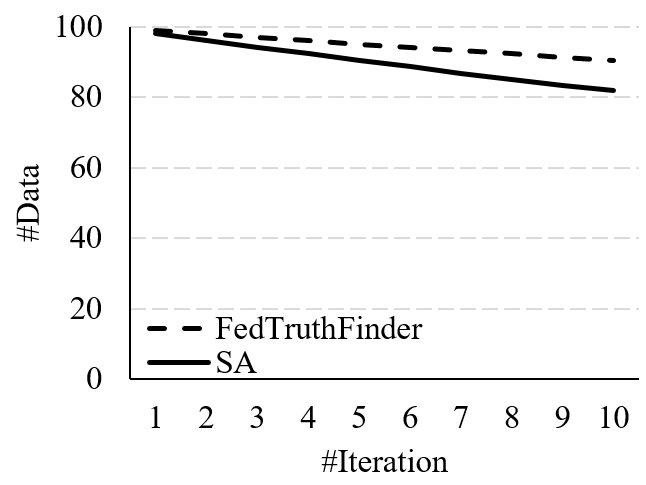
\includegraphics[width=.3\linewidth]{submissions/LeyeWang/fig/data_num_cl0.01.PNG}
			\label{fig:cl0.01}}
		\end{subfigure}
		\begin{subfigure}[$p_l=0.05$]{
			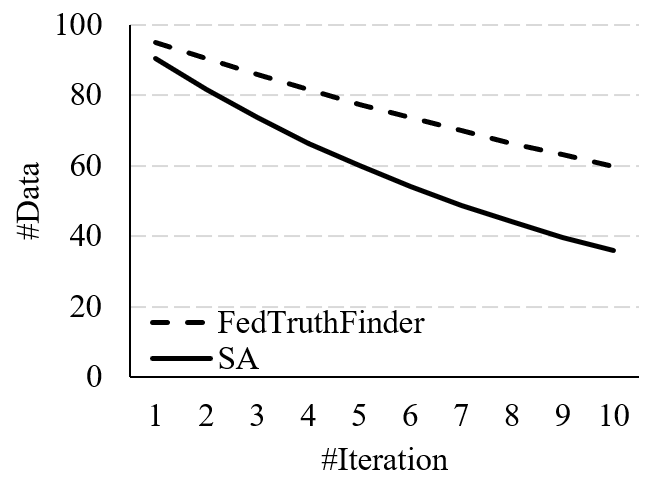
\includegraphics[width=.3\linewidth]{submissions/LeyeWang/fig/data_num_cl0.05.PNG}
			\label{fig:chicago}}
		\end{subfigure}
		\begin{subfigure}[$p_l=0.1$]{
			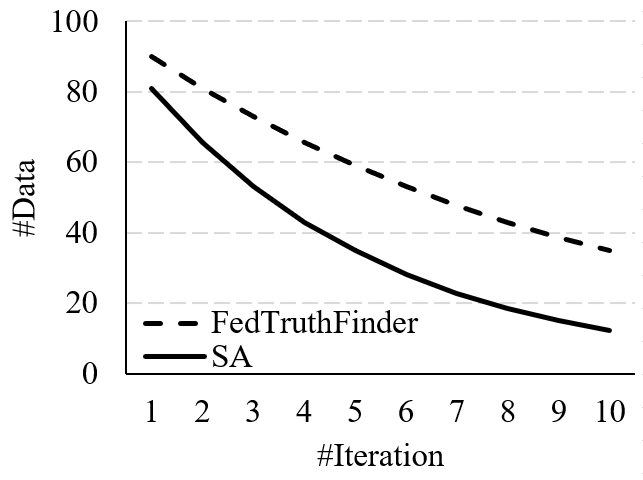
\includegraphics[width=.3\linewidth]{submissions/LeyeWang/fig/data_num_cl0.1.PNG}
			\label{fig:dc}}
		\end{subfigure}
		\caption{Number of data for each event's truth discovery by iterations.}
		\label{fig:num_sensed_data}
\end{figure*}

\begin{figure*}
	\centering
		\begin{subfigure}[$p_l=0.05$]{
			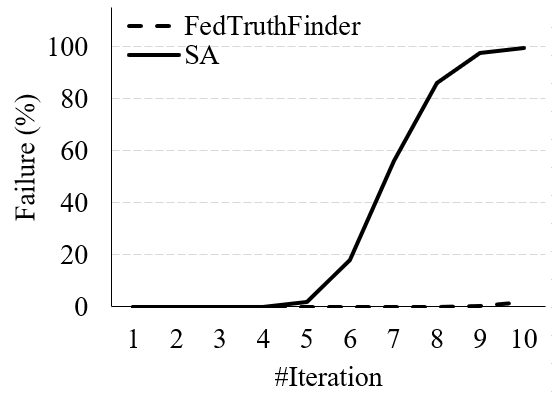
\includegraphics[width=.3\linewidth]{submissions/LeyeWang/fig/failure_cl0.05.PNG}
			}
		\end{subfigure}
		\begin{subfigure}[$p_l=0.1$]{
			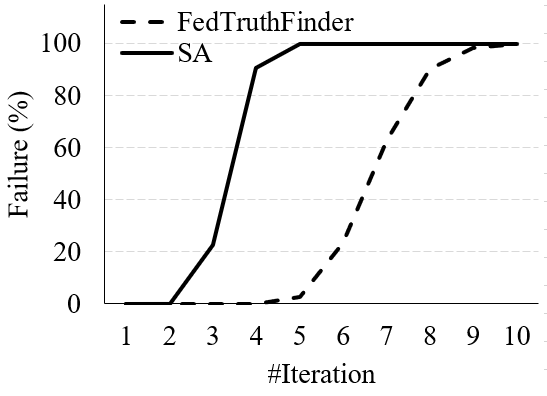
\includegraphics[width=.3\linewidth]{submissions/LeyeWang/fig/failure_cl0.1.PNG}
			}
		\end{subfigure}
		\caption{Failure probability of truth discovery.}
		\label{fig:failure}
\end{figure*}

\vspace{+.5em}
\textbf{Theorem 5.2}. Ranking $h_i$ is equivalent to ranking $\tau_i$.


\subsubsection{Robustness to Connection Loss} We analyze how our secure ranking algorithm can tolerate connection losses. We assume that before Step 2, there is no user connection loss.\footnote{If $u_i$ loses the connection in Step 2 and cannot share $\tau_i^k$ with SSS, then there is no way to rank $u_i$'s position because the server has no $u_i$'s information.}

\vspace{+.5em}
\textbf{Theorem 5.3}. To finish Step 3-5, there needs at least one user online for each group. Suppose that every user has $p_l$ probability to lose connection and there are $n$ users, the success probability $\ge (1-p_l^{\lfloor n/(2t+1) \rfloor})^{2t+1}$.


\vspace{+.5em}
\textbf{Theorem 5.4}. To finish Step 6-8, $\ge t+1$ users need to be online.



\subsubsection{Security} Here, we analyze the security of our mechanism.

\vspace{+.5em}
\textbf{Theorem 5.5} If there are no more than $t$ collusive participants, then these participants cannot recover all the other users' $\tau_i$.






\subsubsection{Complexity} We analyze the algorithm from communication and computation complexity perspectives for participant clients.

\textbf{Communication Complexity - $O(tn)$}. In Step 2, the communication overhead of one participant to send $\tau_i,\tau_i^2,...,\tau_i^{2t+1}$ is $O(t^2)$, while each user received data is $O(tn)$. In Step 3, the complexity is $O(t)$. In Step 5, for sending data, the complexity is $O(n)$; for receiving data, the complexity is $O(tn)$. In Step 7, the complexity is $O(n)$. Combing them together, the communication complexity of the whole process is $O(tn)$ as $t<n$.


\textbf{Computation Complexity - $O(tn)$}. The main computation processes of each client include (1) calculating secret shares for $\tau_i,\tau_i^2,...,\tau_i^{2t+1}$ with $(t+1, 2t+1)$-SSS in Step 2, which is $O(t^2)$, (2) calculating secret shares of $r_k$ in Step 3, which is $O(t)$, (3) computing  $h_i$ in Step 4, which is $O(tn)$, and (4) calculating $h_i'$ in Step 6, which is $O(tn)$. Hence, the final computation complexity is $O(tn)$.


%!TEX root = fed_truth_finder.tex



\section{Evaluation}

\subsection{Numerical Analysis for Connection Loss}
\label{sec:numeric_analysis}

We have theoretically proven that our algorithm can learn the event confidence and trustworthiness ranking like the original centralized algorithms. This experiment then focuses on how the connection loss would impact FedTruthFinder quantitatively, since the unstable mobile network connection is a key characteristic for mobile crowdsensing. A practical mechanism should be able to fight against the unpredictable connection loss.
In general, participants' connection loss may bring two types of negative impacts to the iterative truth discovery algorithm.


\begin{itemize}
	\item \textbf{A small number of sensed data for truth discovery.} While FedTruthFinder can learn an aggregate truth as long as more than $t$ participants are online, the data sources for the truth would be decreased. This would also affect the performance of the learned truth.
	\item \textbf{Possible failure of the whole algorithm.} If a large number of participants lose the connection and only fewer than $t$ participants remain online, then the whole running process of FedTruthFinder would fail and no result can be learned.
\end{itemize}

Specifically, we conduct the numerical analysis for two parts of FedTruthFinder respectively, i.e., event confidence computation and participant trustworthiness ranking. We vary the probability of one participant losing the connection (denoted as $p_l$). If $p_l=0.01$, a participant has 1\% probability of dropping out of the crowdsensing campaign due to one-time connection loss. Then, if a participant needs to connect to the server for $n$ times, it has $1-(1-p_l)^n$ probability to lose the connection. In the experiment, we test $p_l=0.01/0.05/0.1$ to represent good/moderate/bad connection scenarios.




\subsubsection{Event Confidence Computation}

To compare with FedTruthFinder, we consider the state-of-the-art way to do iterative truth discovery with an SSS-based secure aggregation (SA) protocol \cite{Leye-Bonawitz2017PracticalSA,Leye-Xu2019EfficientAP}, denoted as \textit{SA}, which can also tolerate a certain level of participant connection loss.
In brief, SA leverages a double-masking method to ensure that the truth discovery can run when some users lose the connection. However, not like FedTruthFinder which only needs a one-time connection for each participant to finish one iteration of $\rho$-computation, SA needs a two-time connection (double-masking).

Figure~\ref{fig:num_sensed_data} shows the number of sensed data for truth discovery in each iteration for FedTruthFinder and SA (the total number of data is set to 100). Literature has shown that the number of iterations for truth discovery is often smaller than 10 \cite{Leye-yin2008truth} and thus we set the number of iterations up to 10. FedTruthFinder can always obtain more sensed data than SA as FedTruthFinder needs fewer connections. Especially, when the network connection condition is bad ($p_l=0.1$), the performance improvement of FedTruthFinder over SA is more significant.

Figure~\ref{fig:failure} shows the algorithm failure probability (i.e., fewer than $t$ users are online) for FedTruthFinder and SA (we set the number of participants to 100 and $t$ to 50; we do not plot $p_l=0.01$ as both methods are successful almost all the time). FedTruthFinder can significantly reduce the failure probability compared to SA. For example, when the network connection quality is moderate ($p_l = 0.05$), FedTruthFinder has around $99\%$ probability to finish successfully for 10 iterations; however, SA has only around $1\%$ probability. For the bad connection scenario ($p_l = 0.1$), SA will fail with more than $20\%$ probability from iteration 3, while FedTruthFinder can keep working well until iteration 6. This reveals that, even if both FedTruthFinder and SA cannot finish all the ten iterations due to a bad network connection condition, FedTruthFinder can run a larger number of iterations, making the truth more reliable.


\begin{figure*}[t]%[tbhp]
		\centering
		\begin{subfigure}[$p_l=0.01$]{
			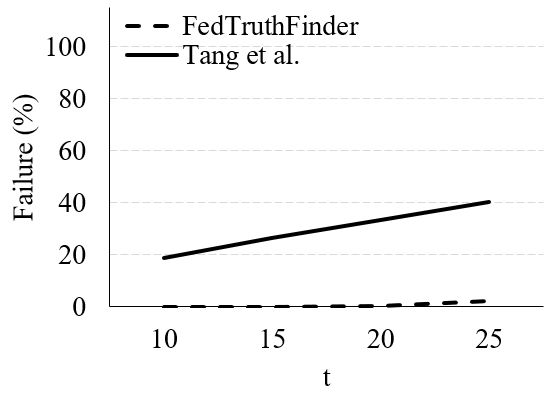
\includegraphics[width=.3\linewidth]{submissions/LeyeWang/fig/fail_trust_0.01.PNG}
			\label{fig:trust_0.01}}
		\end{subfigure}
		\begin{subfigure}[$p_l=0.05$]{
			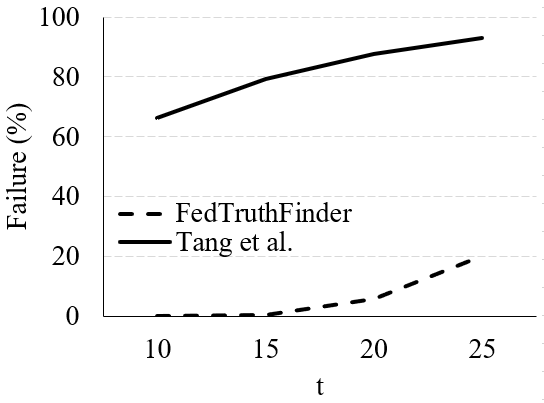
\includegraphics[width=.3\linewidth]{submissions/LeyeWang/fig/fail_trust_0.05.PNG}
			\label{fig:trust_0.05}}
		\end{subfigure}
		\begin{subfigure}[$p_l=0.1$]{
			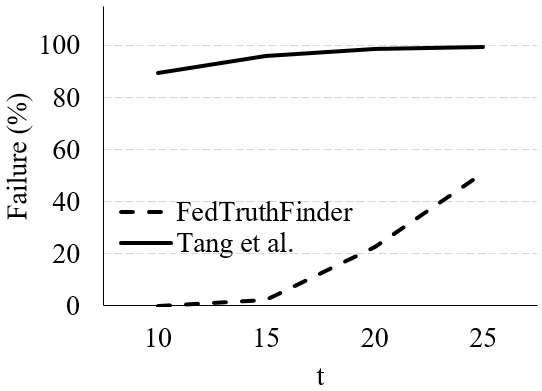
\includegraphics[width=.3\linewidth]{submissions/LeyeWang/fig/fail_trust_0.1.PNG}
			\label{fig:trust_0.1}}
		\end{subfigure}
		\caption{Failure probability of trustworthiness ranking.}
		\label{fig:trust_failure}
\end{figure*}

\begin{figure*}
	\centering
		\begin{subfigure}[Participants number]{
			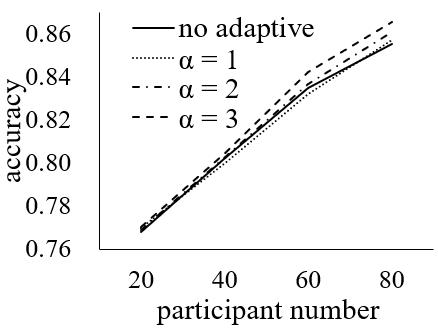
\includegraphics[width=.3\linewidth]{submissions/LeyeWang/fig/truth_acc_traffic_participant_num.PNG}
			\label{fig:acc_vary_participant_num}}
		\end{subfigure}
		\quad
		\begin{subfigure}[Connection loss]{
			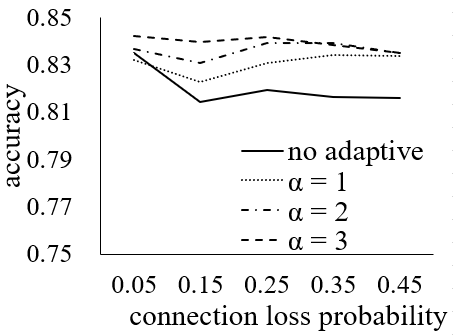
\includegraphics[width=.3\linewidth]{submissions/LeyeWang/fig/truth_acc_traffic_connection_loss.PNG}
			\label{fig:acc_vary_connection_loss}}
		\end{subfigure}
		\caption{Detection accuracy of FedTruthFinder.}
\end{figure*}

\subsubsection{Participant Trustworthiness Rank}

As none of the prior studies have addressed the privacy-preserving trustworthiness ranking problem, we cannot directly find a baseline method to compare. Meanwhile, our proposed trustworthiness ranking algorithm is inspired by the basic idea from \cite{Leye-tang2011secure} while significantly enhancing the capability to tolerate participants' connection loss. To this end, we compare FedTruthFinder and \cite{Leye-tang2011secure} when certain participants lose connections.

In federated trustworthiness ranking, $t$ is the key parameter related to how many user groups are created, which significantly impacts the algorithm success probability (Theorem 5.3). Suppose the total number of users is 100, we set $t=10/15/20/25$. The algorithm failure probability is shown in Figure~\ref{fig:trust_failure}. With the increase of $t$, the failure probability of FedTruthFinder rises. This fits our expectation as a larger $t$ means that more user groups are generated and the user number per group is reduced. As FedTruthFinder needs at least one user online for each group, smaller user number per group means that the robustness against connection loss is weakened, leading to higher failure probability. Compared to \cite{Leye-tang2011secure}, our algorithm significantly increases the success probability when connection is unstable. When $p_l = 0.1$ and $t=10$, the failure probability of our ranking algorithm is 0.04\%, but \cite{Leye-tang2011secure} is 96.18\%.
Hence, our algorithm could be an appropriate choice for ranking crowdsensing participants' trustworthiness scores considering the unstable mobile network connection environment.



\subsection{Evaluation of Traffic Light Detection}

We also test FedTruthFinder for traffic light detection, a representative crowdsensing task \cite{Leye-ouyang2015truth,Leye-wang2013credibility}. We focus on the truth discovery accuracy and the runtime efficiency of FedTruthFinder, which has not been evaluated in the previous numerical analysis.


\begin{figure}[t]
	\centering
	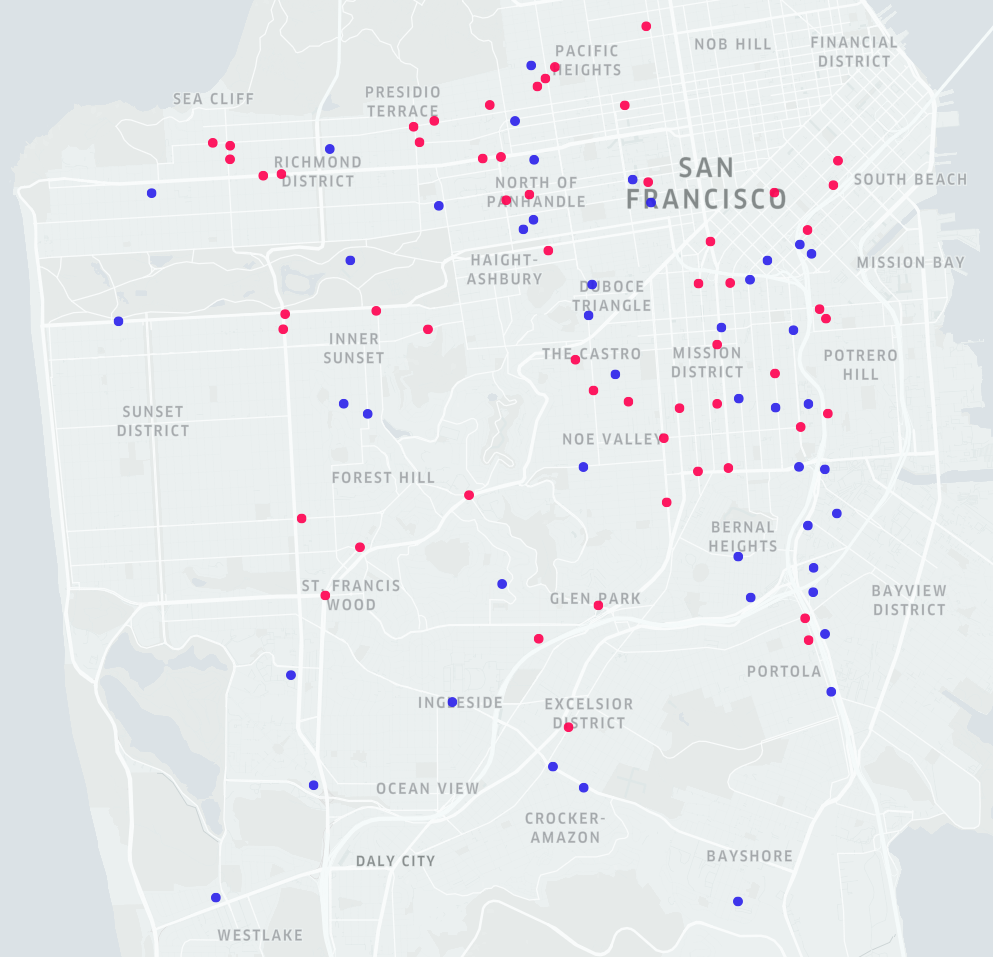
\includegraphics[width=.8\linewidth]{submissions/LeyeWang/fig/traffic_light_map.png}
	\caption{Traffic light event locations (red: true; blue: false). The red points represent the true event locations (i.e, with traffic lights) and the blue points mean the false event locations.}
	\label{fig:traffic_light_map}
\end{figure}

\subsubsection{Data and Tasks} To evaluate FedTruthFinder on the traffic light detection task, we leverage a real-life open dataset including taxis' trajectories. Specifically, the dataset contains time-stamped GPS trajectories from 536 taxis in San Francisco, U.S. in one month of 2008 \cite{Leye-epflmobility}. Following \cite{Leye-ouyang2015truth}, we manually label 96 traffic light detection event positions using the Street View of Google Maps (Figure~\ref{fig:traffic_light_map}). Then, we randomly select some taxis as participants; their trajectories in the dataset are used to simulate their activities --- if a taxi stops around an event's location, it may report the data. The report error rate (indicating trustworthiness) of each taxi is randomized in $[0,0.5]$. The default participant number is 60 and the connection loss probability is 0.05. The event confidence function is set to `logistic' as it performs better than `sum'. $t$ in SSS is set to half of the total participant number. To increase the randomness, each taxi randomly reports 20\% of the events, and then each setting of the experiment is repeated by 50 times.

\subsubsection{Experiment Platform} Our platform is an Alibaba cloud server with CPU of Intel Xeon Platinum 8163 (12 cores, 2.5GHz) and 24GB memory. The operating system is Ubuntu 20.04. FedTruthFinder is implemented by \textit{Rust} 1.56. \textit{Docker}\footnote{https://www.docker.com/} is adopted to simulate the crowdsensing server and participants.


\subsubsection{Truth Discovery Accuracy} Figure \ref{fig:acc_vary_participant_num} and \ref{fig:acc_vary_connection_loss} plot the accuracy regarding the number of participants and connection loss probability, respectively. Specifically, we compare FedTruthFinder with and without the adaptive truth updating technique (Sec.~\ref{sub:adaptive_truth_updating}). For the adaptive updating, we try $\alpha=1/2/3$ (Eq.~\ref{eq:adaptive_weight}), and find $\alpha=3$ performs the best. The adaptive updating ($\alpha=3$) can consistently improve the accuracy with different participant numbers and connection losses. Specifically, with more participants and higher connection losses, the improvement is more significant. When the connection loss probability increases, the accuracy decreases gradually. This again verifies the effectiveness of FedTruthFinder over SA \cite{Leye-Xu2019EfficientAP} --- FedTruthFinder reduces the communication times per truth discover iteration compared to SA, which is conceptually equivalent to the reduction of connection losses in practice.


\begin{figure}[t]%[tbhp]
	\centering
	\begin{subfigure}[Data transmission]{
		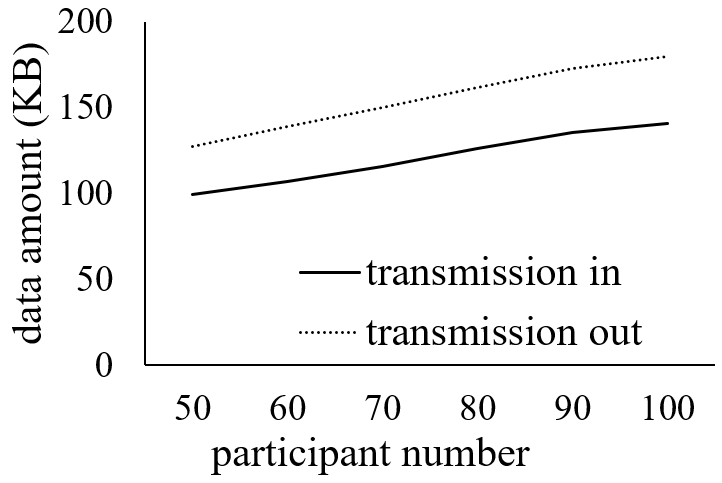
\includegraphics[width=.3\linewidth]{submissions/LeyeWang/fig/data_transmission_traffic.PNG}
		\label{fig:data_transmission}}
	\end{subfigure}
	\
	\begin{subfigure}[Domputation time]{
		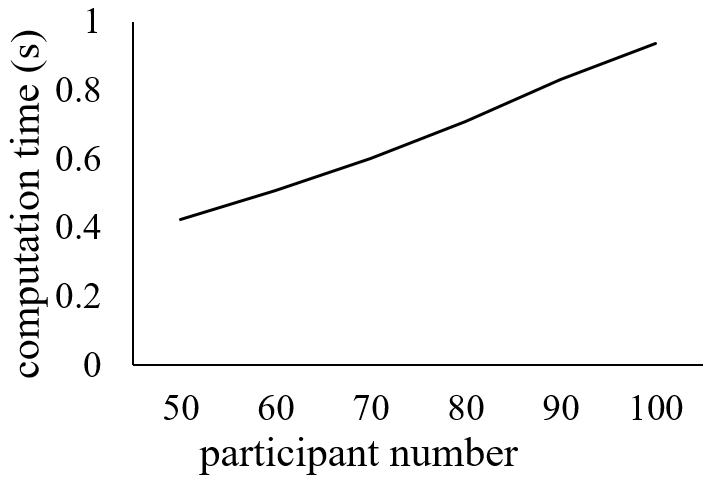
\includegraphics[width=.3\linewidth]{submissions/LeyeWang/fig/computation_time_traffic.PNG}
		\label{fig:computation_time}}
	\end{subfigure}
	\caption{Runtime efficiency of FedTruthFinder.}
\end{figure}

\subsubsection{Runtime Efficiency} Figure~\ref{fig:data_transmission} and \ref{fig:computation_time} record each participant's data transmission amount and computation time, respectively. Note that the computation time is mostly spent in the truth finding step, while the trustworthiness ranking takes only $\sim$0.01s. The results show that the data transmission amount and computation time are both small, verifying the practicality of FedTruthFinder.



\section{Related Work}



Truth discovery is a traditional research direction as we may often receive diverse and even conflicting information about one event \cite{Leye-li2016survey}. In the pioneering research \cite{Leye-yin2008truth}, authors discuss the truth discovery problem when there are many conflicting facts about one subject on different websites.
Besides information from websites, truth discovery is also important in many other areas such as social sensing \cite{Leye-wang2012truth} and crowdsourcing \cite{Leye-li2014the,Leye-Whitehill2009WhoseVS}.

Mobile crowdsensing \cite{Leye-zhang20144w1h}, as a particular type of crowdsourcing that needs workers to do location-based sensing tasks, would also face the truth discovery problem \cite{Leye-Wang2014SurrogateMS}. Meanwhile, privacy protection is also an important issue to consider in crowdsensing, especially for location privacy \cite{Leye-han2021hidden,Leye-wang2016differential,Leye-Wang2017LocationPT,Leye-Wang2019PersonalizedPT,Leye-Wang2020SparseMC,Leye-Wang2019MobileCT}. Most prior research focuses on protecting crowdsensing participants' location privacy in task allocation \cite{Leye-Wang2017LocationPT,Leye-Wang2019PersonalizedPT,Leye-Wang2019MobileCT} or for particular crowdsensing tasks such as missing data inference \cite{Leye-wang2016differential,Leye-Wang2020SparseMC}.

Recently, some studies investigate the privacy-preserving truth discovery in crowdsensing \cite{Leye-Miao2015CloudEnabledPT,Leye-Miao2017ALP,Leye-Miao2019PrivacyPreservingTD,Leye-Zhang2021ReliableAP,Leye-ZHANG2020101848,Leye-Xu2019EfficientAP}. One research direction is applying data perturbation methods such as differential privacy to participants' sensed data \cite{Leye-Li2018AnET,Leye-Li2020TowardsDP}, but these methods degrade the truth finding accuracy. Another research direction follows the federated learning \cite{Leye-yang2019federated} paradigm that participants' raw data will not be directly sent to the server with certain encryption techniques, while the aggregation results (i.e., detected truths) can be accurately learned. However, the existing privacy-preserving truth discovery methods usually suffer from certain assumptions which may not stand in reality, e.g., online/non-concluding participants \cite{Leye-Miao2015CloudEnabledPT,Leye-Miao2017ALP,Leye-Miao2019PrivacyPreservingTD}, or third-party non-concluding servers \cite{Leye-Zhang2021ReliableAP,Leye-ZHANG2020101848}.
Moreover, no prior work considers hiding participants' completed tasks or tracking participants' trustworthiness in a privacy-preserving manner, which has been addressed by our work.

\begin{table*}[t]
	\footnotesize
	\centering
	\caption{Comparison of our work and representative related work. (NTP: No Third Party, AT: Assess Trustworthiness,  CA: Collusion Attacks)}
	\label{tab:related_work}
	\begin{tabular}{@{}lccccccc@{}}
		\toprule
		\textbf{} &
		\multicolumn{2}{c}{\textbf{Privacy Protection}}
		&
		\textbf{NTP} &
		\textbf{AT} &
		\multicolumn{2}{c}{\textbf{Connection Loss}} & \textbf{CA} \\
		&
		\textit{Sensed Data} &
		\textit{Completed Tasks}
		&
		&
		& \textit{Fault Tolerance} & \textit{Bias Avoidance}
		& \\
		\midrule
		\cite{Leye-Miao2017ALP} & $\surd$  & $\times$ & $\times$ & $\times$  & $\times$ & $\times$ & $\times$ \\
		\cite{Leye-Zheng2018LearningTT} & $\surd$  & $\times$ & $\times$ & $\times$  & $\surd$ & $\times$ & $\times$ \\
		\cite{Leye-Miao2019PrivacyPreservingTD}  & $\surd$  & $\times$ & $\surd$ & $\times$  & $\surd$ & $\times$  & $\times$ \\
		\cite{Leye-Xu2019EfficientAP}  & $\surd$ & $\times$ & $\surd$ & $\times$ & $\surd$ & $\times$ & $\surd$ \\
		\cite{Leye-Zheng2020PrivacyAwareAE} & $\surd$ & $\times$ & $\surd$ & $\times$ & $\surd$ & $\times$ & $\surd$ \\
		\cite{Leye-Zhang2021ReliableAP}  & $\surd$ & $\times$ & $\times$ & $\times$ & $
		\surd$ & $\times$ & $\times$\\
		Our Work & $\surd$ & $\surd$ & $\surd$ & $\surd$ & $\surd$ & $\surd$ & $\surd$ \\ \bottomrule
	\end{tabular}
\end{table*}


Table \ref{tab:related_work} summarizes the characteristics of our work and representative related work published in top venues recently. In particular, our work is the \textbf{first} privacy-preserving crowdsensing truth discovery research that considers (i) \textit{providing a feasible solution to participant trustworthiness assessment} when the trustworthiness scores are not revealed, and (ii) \textit{hiding participants' completed tasks} to provide stronger privacy protection. Moreover, when dealing with the connection loss during the iterative crowdsensing truth discovery process, our work (i) proposes an adaptive event confidence updating function to reserve the data contributions of drop-out participants to avoid the truth bias toward alive participants, and (ii) designs an SSS-based scheme to defend against participants' collusion attacks while ensuring the high communication efficiency.


%\section{Future Work}
%
%As a pioneering attempt to solve the truth discovery problem in crowdsensing, our research still has certain limitations and points out some future opportunities.
%
%\textbf{Multi-class and Continuous-value Event Sensing}. In this work, we focus on binary event sensing. Naturally, our method can be extended to multi-class event sensing. Besides, sometimes we need to sense continuous value for a certain event (e.g., temperature). We will also study this in the future.
%
%%\textbf{Homomorphic Encryption-enabled Truth Discovery}. In FL systems, two widely adopted security mechanisms are homomorphic encryption (HE) and secure multi-party computation (SMC) \cite{Leye-yang2019federated}. Shamir's secret sharing is one type of SMC, which we rely on to build FedTruthFinder. HE may be another technical route to reach the goal. Currently, we do not choose HE because its computation efficiency is 10-100 times slower than non-HE computation. Some pioneering efforts have been devoted to developing privacy-preserving truth discovery systems with HE. Due to the large computation burden, these studies only let two non-colluding powerful servers to do HE computation instead of letting each client do computation in a federated (distributed) manner \cite{Leye-Tang2018NonInteractivePT,Zheng2018LearningTT}. However, finding two non-colluding servers are not so easy \cite{Leye-Bonawitz2017PracticalSA}.
%
%
%% they assume there need to be two non-colluding parties who take all the computation tasks.
%
%%Currently, we do not choose HE because its computation efficiency is 10-100 times slower than non-HE computation. Recently, HE tools have developed rapidly \cite{Leye-sealcrypto}, and we believe HE-enabled truth discovery is a promising direction.
%
%\textbf{Other Truth Discovery Algorithms}. Besides the iterative truth discovery algorithm discussed in this paper, there are also other state-of-the-art truth discovery algorithms, such as optimization-based methods \cite{Leye-Li2014ACA,Li2015OnTD} and graphical model-based methods \cite{Leye-Pasternack2013LatentCA,Zhao2012ABA}. A comprehensive survey on truth discovery algorithms can be referred to \cite{Leye-li2016survey}. In the future, we will study whether our methods can be adapted to more truth discovery algorithms.
%
%\textbf{Against More Serious Attack Scenarios}. In this work, we assume that all the users are semi-honest, i.e., they will follow the protocol to compute and upload the corresponding data. In a more competitive setting, users can be malicious and upload some wrong data for attacking other users' privacy. We will discuss the solutions under such conditions in the future.
%
%\textbf{Missing Negative Sensed Data}. For some crowdsensing applications, users would only upload the positive sensed data ($e_j=1$). The truth discovery algorithms need to be refined as negative sensed data ($e_j=0$) are implicit. We will try to develop the federated version of such truth discovery algorithms in our future work.
%
%\textbf{Deployment on Smartphones}. In this work, we focus on the algorithmic design. In the future, we will implement the algorithm and deploy it to smartphones to further test its communication costs, energy consumption, etc. We will try to find practical guidelines to deploy such a federated crowdsensing truth discovery mechanism.

\section{Conclusion}

In this paper, we propose \textit{FedTruthFinder}, a crowdsensing federated truth discovery mechanism that can not only find aggregate truth from multiple participants' sensed data, but also rank participants' trustworthiness in a privacy-preserving manner. The primary characteristic of FedTruthFinder is its capability to tolerate network connection loss of participants in both event confidence calculation and participant trustworthiness ranking. As a byproduct, our proposed federated ranking algorithm can also serve other applications when the privacy-preserving data ranking is needed and the network connections are unstable.
Following most related papers, this work assumes participants to be semi-honest; in the future, we would explore the more challenging scenario that participants may behave maliciously.%To the best of our knowledge, FedTruthFinder is the best privacy-preserving truth discovery mechanism for crowdsensing regarding the robustness against participants' unpredictable connection loss.



%\onecolumn
%\appendix
\section{Appendix}

\subsection{Theoretical Proof}

%\subsubsection{Correctness} We first prove that the correctness of our secure leader-board algorithm.
%
%\vspace{+.5em}
%\textbf{Lemma 5.1}. $\sum_{k=1}^{2t+1} r_k(x)\tau_{i_k}(x)$ can be represented as:
%$$h_{i}+a_{i1}x+a_{i2}x^2+...+a_{i2t}x^{2t}$$
%where $h_i=\sum_{k=1}^{2t+1} r_k\tau_i^k$. \cite{Leye-tang2011secure}

\textbf{Proof of Lemma 5.1}. It is clear that,
\begin{equation}
	\sum_{k=1}^{2t+1} r_k(0)\tau_{i_k}(0) = \sum_{k=1}^{2t+1} r_k\tau_i^k
\end{equation}
Besides, both $r_k(x)$ and $\tau_{i_k}(x)$ are $t$-degree polynomials, and thus the degree of $\sum_k r_k(x)\tau_{i_k}(x)$ is $2t$.$\qed$

\vspace{+.5em}
%\textbf{Theorem 5.1}. With $t+1$ participants' $h'_i(k)$, we can recover $h_i$.

\noindent \textbf{Proof of Theorem 5.1}. With Lemma 5.1, for $N$ ($=2t+1$) groups, $\gamma(gid(u_j))
=\sum_{k=1}^{2t+1} r_k(gid(u_j)) \tau_{i_k}(gid(u_j))$ (Step 4) is:

\[
\small
\left(\begin{array}{ccccc}
	1 &    1 & 1^2 & ...  & 1^{2t} \\
	1 &    2 & 2^2 & ... & 2^{2t}\\
	... & ... & ... & ...& ...\\
	1 & N & N^2 & ... & N^{2t}\\
\end{array}\right)
\left(\begin{array}{c}
	h_i    \\
	a_{i1}    \\
	... \\
	a_{i2t} \\
\end{array}\right)
=
\left(\begin{array}{c}
	\gamma(1)    \\
	\gamma(2)    \\
	... \\
	\gamma(N) \\
\end{array}\right)
\]
then,
\[
\small
\left(\begin{array}{c}
	h_i    \\
	a_{i1}    \\
	... \\
	a_{i2t} \\
\end{array}\right)
=
\left(\begin{array}{ccccc}
	1 &    1 & 1^2 & ...  & 1^{2t} \\
	1 &    2 & 2^2 & ... & 2^{2t}\\
	... & ... & ... & ...& ...\\
	1 & N & N^2 & ... & N^{2t}\\
\end{array}\right)^{-1}
\left(\begin{array}{c}
	\gamma(1)    \\
	\gamma(2)    \\
	... \\
	\gamma(N) \\
\end{array}\right)
\]
so,
$$h_i=\sum_{g=1}^{N} \lambda(g)\gamma(g)$$

In Step 5, $h_i(g)=\lambda(g)\gamma(g)$ is shared with $(t+1,n)$-SSS to all the participants from every group $g \in [1, 2t+1]$. Hence, according to the additive homomorphism property of SSS \cite{Leye-shamir1979share}, we can easily recover $h_i$ by receiving $t+1$ participants'  $h'_i(k) = \sum_{g=1}^{2t+1} h_i(g, k)$.$\qed$

\vspace{+.5em}
%\textbf{Theorem 5.2}. Ranking $h_i$ is equivalent to ranking $\tau_i$.

\noindent \textbf{Proof of Theorem 5.2}. As $\tau_i>0$ and $r_k>0$, $h_i=\sum_k r_k\tau_i^k$ will keep the same ranking as $\tau_i$.$\qed$

%\subsubsection{Robustness to Connection Loss} While mobile users may lose network connections during a crowdsensing campaign, we analyze how our secure ranking algorithm can tolerate connection losses. Without the loss of generalizability, we assume that before Step 2, there is no user connection loss.\footnote{If $u_i$ loses the connection in Step 2 and cannot share $\tau_i^k$ with SSS, then there is no way to rank $u_i$'s position because the server has no $u_i$'s information. So we only consider the users who establish the connections to share $\tau_i^k$ in Step 2 for ranking.}

\vspace{+.5em}
%\textbf{Theorem 5.3}. To finish Step 3-5, there needs at least one user online for each group. Suppose that every user has $p_l$ probability to lose connection and there are totally $n$ users, the success probability $\ge (1-p_l^{\lfloor n/(2t+1) \rfloor})^{2t+1}$.

\noindent \textbf{Proof of Theorem 5.3}. For Step 3 to 5, if there is at least one user in every group, then the process can continue. So the probability of failure incurred by one specific group $g$ is all the users in $g$ losing the connections, i.e., $p^{n_g} \le p_l^{\lfloor n/(2t+1) \rfloor}$ ($n_g$ is the user number in $g$). So for $g$, the probability of at least one user online $\ge 1-p_l^{\lfloor n/(2t+1) \rfloor}$. With $2t+1$ groups, the success probability $\ge (1-p_l^{\lfloor n/(2t+1) \rfloor})^{2t+1}$.$\qed$
%For Step 6 to 8, if at least $t'$ users have connections, then the server can recover $h_i$. Hence, the probability of failure is more than $N-t'$ users losing connections:
%$$p^{N-t'+1}$$

\vspace{+.5em}
%\textbf{Theorem 5.4}. To finish Step 6-8, $\ge t+1$ users need to be online.

\noindent \textbf{Proof of Theorem 5.4}. This is based on the property of $(t+1, n)$-SSS in Step 5.$\qed$


\vspace{+.5em}
%\textbf{Theorem 5.5} If there are no more than $t$ collusive participants, then these participants cannot recover all the other users' $\tau_i$.

\noindent \textbf{Proof of Theorem 5.5}. In Step 2, $\tau_i^k (k=1...2t+1)$ is shared with $(t+1, 2t+1)$-SSS. So, if $t$ participants collude, they can get at most $t\cdot(2t+1)$ equations when $t$ participants are from $t$ groups. However, the number of unknown parameters (including $\tau_i$ and $t$ random coefficients for sharing each $\tau_i^k$) is $t\cdot(2t+1)+1$. Hence, these $t$ collusive participants cannot recover other participants' $\tau_i$.$\qed$

\subsection{Mechanism Extension to Multi-class and Continuous-value Events}



\textbf{Multi-class Events}. For a multi-class event ($m$ classes), we can see it as $m$ binary events, so that our method can be directly applied.

\noindent \textbf{Continuous-value Events}. For continuous-value events, following the literature, we may adopt other proper event confidence and participant trustworthiness updating functions such as CRH \cite{Leye-Xu2019EfficientAP,Leye-Zheng2020PrivacyAwareAE}. Specifically, suppose that the discovered truth sensed value of a continuous event $e_j$ is $\rho_j$, and $u_i$'s sensed data of $e_j$ is $\hat \rho_{ij}$, then the event truth (confidence) and participant trustworthiness updating functions  can be:
\begin{equation}
	\rho_j = \frac{\sum_{u_i \in \mathcal U_{e_j}}\tau_i \cdot \hat \rho_{ij}}{\sum_{u_i \in \mathcal U_{e_j}}\tau_i}
	\label{eq:rho_function_cont}
\end{equation}
\begin{equation}
	\tau_i = \log(\sum_{u_i \in \mathcal U} \sum_{e_j \in \mathcal E_{u_i}} \frac{(\rho_j- \hat \rho_{ij})^2}{|\mathcal E_{u_i}|}) - \log(\sum_{e_j \in \mathcal E_{u_i}} \frac{(\rho_j- \hat \rho_{ij})^2}{|\mathcal E_{u_i}|})
	\label{eq:tau_function_cont}
\end{equation}
where $\mathcal U_{e_j}$ is the set of users who sense $e_j$, and $\mathcal E_{u_i}$ is the set of events that $u_i$ has sensed. For $\rho$-computation, following Sec.~\ref{sub:basic_rho_computation}, we can just adapt $d_{ij}$ and $s_{ij}$ according to Eq.~\ref{eq:rho_function_cont} (the participant $u_i \not \in \mathcal U_{e_j}$ can still send $d_{ij}=s_{ij}=0$ to protect her task completion information). For $\tau$-computation, Eq.~\ref{eq:tau_function_cont} requires $\sum_{u_i \in \mathcal U} \sum_{e_j \in \mathcal E_{u_i}} \frac{(\rho_j- \hat \rho_{ij})^2}{|\mathcal E_{u_i}|}$, which can be done with the same SSS-based method as $\rho$-computation. In particular, each participant $u_i$ can send $\sum_{e_j \in \mathcal E_{u_i}} \frac{(\rho_j- \hat \rho_{ij})^2}{|\mathcal E_{u_i}|}$ by secret shares, and then the server can compute the sum in a privacy-preserving manner. In a word, for continuous-value events, our mechanism can still work without revealing each participant's raw sensed data and completed tasks.







%%
%% The next two lines define the bibliography style to be used, and
%% the bibliography file.

\begin{thebibliography}{10}

\bibitem{Leye-Bonawitz2017PracticalSA}
K.~Bonawitz, V.~Ivanov, B.~Kreuter, A.~Marcedone, H.~McMahan, S.~Patel,
  D.~Ramage, A.~Segal, and K.~Seth.
\newblock Practical secure aggregation for privacy-preserving machine learning.
\newblock {\em CCS}, 2017.

\bibitem{Leye-chai2020secure}
D.~Chai, L.~Wang, K.~Chen, and Q.~Yang.
\newblock Secure federated matrix factorization.
\newblock {\em IEEE Intelligent Systems}, 2020.

\bibitem{Leye-ganti2011mobile}
R.~K. Ganti, F.~Ye, and H.~Lei.
\newblock Mobile crowdsensing: current state and future challenges.
\newblock {\em IEEE Communications Magazine}, 49(11):32--39, 2011.

\bibitem{Leye-han2021hidden}
X.~Han, L.~Wang, and W.~Fan.
\newblock Is hidden safe? location protection against machine-learning
  prediction attacks in social networks.
\newblock {\em MIS Quarterly}, 45(2):821--858, 2021.

\bibitem{Leye-konevcny2016federated}
J.~Kone{\v{c}}n{\`y}, H.~B. McMahan, F.~X. Yu, P.~Richt{\'a}rik, A.~T. Suresh,
  and D.~Bacon.
\newblock Federated learning: Strategies for improving communication
  efficiency.
\newblock {\em arXiv:1610.05492}, 2016.

\bibitem{Leye-li2014the}
H.~{Li}, B.~{Zhao}, and A.~{Fuxman}.
\newblock The wisdom of minority: discovering and targeting the right group of
  workers for crowdsourcing.
\newblock In {\em WWW}, pages 165--176, 2014.

\bibitem{Leye-li2016survey}
Y.~Li, J.~Gao, C.~Meng, Q.~Li, L.~Su, B.~Zhao, W.~Fan, and J.~Han.
\newblock A survey on truth discovery.
\newblock {\em SIGKDD Explor. Newsl.}, 17(2):1–16, Feb. 2016.

\bibitem{Leye-Li2018AnET}
Y.~Li, C.~Miao, L.~Su, J.~Gao, Q.~Li, B.~Ding, Z.~Qin, and K.~Ren.
\newblock An efficient two-layer mechanism for privacy-preserving truth
  discovery.
\newblock {\em KDD}, 2018.

\bibitem{Leye-Li2020TowardsDP}
Y.~Li, H.~Xiao, Z.~Qin, C.~Miao, L.~Su, J.~Gao, K.~Ren, and B.~Ding.
\newblock Towards differentially private truth discovery for crowd sensing
  systems.
\newblock {\em ICDCS}, pages 1156--1166, 2020.

\bibitem{Leye-liu2020secure}
Y.~{Liu}, Y.~{Kang}, C.~{Xing}, T.~{Chen}, and Q.~{Yang}.
\newblock A secure federated transfer learning framework.
\newblock {\em IEEE Intelligent Systems}, 35(4):70--82, 2020.

\bibitem{Leye-ma2014opportunities}
H.~Ma, D.~Zhao, and P.~Yuan.
\newblock Opportunities in mobile crowd sensing.
\newblock {\em IEEE Communications Magazine}, 52(8):29--35, 2014.

\bibitem{Leye-meng2015truth}
C.~Meng, W.~Jiang, Y.~Li, J.~Gao, L.~Su, H.~Ding, and Y.~Cheng.
\newblock Truth discovery on crowd sensing of correlated entities.
\newblock In {\em Proceedings of the 13th ACM Conference on Embedded Networked
  Sensor Systems}, pages 169--182, 2015.

\bibitem{Leye-Miao2015CloudEnabledPT}
C.~Miao, W.~Jiang, L.~Su, Y.~Li, S.~Guo, Z.~Qin, H.~Xiao, J.~Gao, and K.~Ren.
\newblock Cloud-enabled privacy-preserving truth discovery in crowd sensing
  systems.
\newblock In {\em SenSys}, 2015.

\bibitem{Leye-Miao2019PrivacyPreservingTD}
C.~Miao, W.~Jiang, L.~Su, Y.~Li, S.~Guo, Z.~Qin, H.~Xiao, J.~Gao, and K.~Ren.
\newblock Privacy-preserving truth discovery in crowd sensing systems.
\newblock {\em ACM Transactions on Sensor Networks}, 15:1 -- 32, 2019.

\bibitem{Leye-Miao2017ALP}
C.~Miao, L.~Su, W.~Jiang, Y.~Li, and M.~Tian.
\newblock A lightweight privacy-preserving truth discovery framework for mobile
  crowd sensing systems.
\newblock {\em INFOCOM}, pages 1--9, 2017.

\bibitem{Leye-ouyang2015truth}
R.~W. Ouyang, M.~Srivastava, A.~Toniolo, and T.~J. Norman.
\newblock Truth discovery in crowdsourced detection of spatial events.
\newblock {\em IEEE transactions on knowledge and data engineering},
  28(4):1047--1060, 2015.

\bibitem{Leye-Peng2018DataQG}
D.~Peng, F.~Wu, and G.~Chen.
\newblock Data quality guided incentive mechanism design for crowdsensing.
\newblock {\em IEEE Transactions on Mobile Computing}, 17:307--319, 2018.

\bibitem{Leye-epflmobility}
M.~Piorkowski, N.~Sarafijanovic-Djukic, and M.~Grossglauser.
\newblock {CRAWDAD} dataset epfl/mobility (v. 2009-02-24).
\newblock Downloaded from \url{https://crawdad.org/epfl/mobility/20090224},
  Feb. 2009.

\bibitem{Leye-Primault2019TheLR}
V.~Primault, A.~Boutet, S.~B. Mokhtar, and L.~Brunie.
\newblock The long road to computational location privacy: A survey.
\newblock {\em IEEE Communications Surveys \& Tutorials}, 21:2772--2793, 2019.

\bibitem{Leye-Reddy2010ExaminingMF}
S.~Reddy, D.~Estrin, M.~Hansen, and M.~Srivastava.
\newblock Examining micro-payments for participatory sensing data collections.
\newblock {\em UbiComp}, 2010.

\bibitem{Leye-shamir1979share}
A.~Shamir.
\newblock How to share a secret.
\newblock {\em Communications of the ACM}, 22(11):612--613, 1979.

\bibitem{Leye-tang2011secure}
C.~Tang, G.~Shi, and Z.~Yao.
\newblock Secure multi-party computation protocol for sequencing problem.
\newblock {\em SCIENTIA SINICA Informationis}, 41(7):789--797, 2011.

\bibitem{Leye-Tang2018NonInteractivePT}
X.~Tang, C.~Wang, X.~Yuan, and Q.~Wang.
\newblock Non-interactive privacy-preserving truth discovery in crowd sensing
  applications.
\newblock {\em INFOCOM}, pages 1988--1996, 2018.

\bibitem{Leye-Wang2014SurrogateMS}
D.~Wang, T.~Abdelzaher, and L.~M. Kaplan.
\newblock Surrogate mobile sensing.
\newblock {\em IEEE Communications Magazine}, 52:36--41, 2014.

\bibitem{Leye-wang2013credibility}
D.~Wang, L.~Kaplan, T.~Abdelzaher, and C.~C. Aggarwal.
\newblock On credibility estimation tradeoffs in assured social sensing.
\newblock {\em IEEE Journal on Selected Areas in Communications},
  31(6):1026--1037, 2013.

\bibitem{Leye-wang2012truth}
D.~Wang, L.~Kaplan, H.~Le, and T.~Abdelzaher.
\newblock On truth discovery in social sensing: A maximum likelihood estimation
  approach.
\newblock In {\em IPSN}, pages 233--244, 2012.

\bibitem{Leye-Wang2017LocationPT}
L.~Wang, D.~Yang, X.~Han, T.~Wang, D.~Zhang, and X.~Ma.
\newblock Location privacy-preserving task allocation for mobile crowdsensing
  with differential geo-obfuscation.
\newblock {\em WWW}, 2017.

\bibitem{Leye-Wang2019MobileCT}
L.~Wang, D.~Yang, X.~Han, D.~Zhang, and X.~Ma.
\newblock Mobile crowdsourcing task allocation with differential-and-distortion
  geo-obfuscation.
\newblock {\em IEEE Transactions on Dependable and Secure Computing},
  18:967--981, 2021.

\bibitem{Leye-Wang2020SparseMC}
L.~Wang, D.~Zhang, D.~Yang, B.~Y. Lim, X.~Han, and X.~Ma.
\newblock Sparse mobile crowdsensing with differential and distortion location
  privacy.
\newblock {\em IEEE Transactions on Information Forensics and Security},
  15:2735--2749, 2020.

\bibitem{Leye-wang2016differential}
L.~Wang, D.~Zhang, D.~Yang, B.~Y. Lim, and X.~Ma.
\newblock Differential location privacy for sparse mobile crowdsensing.
\newblock In {\em ICDM}, pages 1257--1262. IEEE, 2016.

\bibitem{Leye-Wang2021AST}
T.~Wang, C.~Lv, C.~Wang, F.~Chen, and Y.~Luo.
\newblock A secure truth discovery for data aggregation in mobile crowd
  sensing.
\newblock {\em Secur. Commun. Networks}, 2021:2296386:1--2296386:15, 2021.

\bibitem{Leye-Wang2019PersonalizedPT}
Z.~Wang, J.~Hu, R.~Lv, J.~Wei, Q.~Wang, D.~Yang, and H.~Qi.
\newblock Personalized privacy-preserving task allocation for mobile
  crowdsensing.
\newblock {\em IEEE Transactions on Mobile Computing}, 18:1330--1341, 2019.

\bibitem{Leye-Whitehill2009WhoseVS}
J.~Whitehill, P.~Ruvolo, T.~Wu, J.~Bergsma, and J.~Movellan.
\newblock Whose vote should count more: Optimal integration of labels from
  labelers of unknown expertise.
\newblock In {\em NeurIPS}, 2009.

\bibitem{Leye-Xu2019EfficientAP}
G.~Xu, H.~Li, S.~Liu, M.~Wen, and R.~Lu.
\newblock Efficient and privacy-preserving truth discovery in mobile crowd
  sensing systems.
\newblock {\em IEEE Transactions on Vehicular Technology}, 68:3854--3865, 2019.

\bibitem{Leye-yang2019federated}
Q.~Yang, Y.~Liu, T.~Chen, and Y.~Tong.
\newblock Federated machine learning: Concept and applications.
\newblock {\em ACM Transactions on Intelligent Systems and Technology},
  10(2):12, 2019.

\bibitem{Leye-yin2008truth}
X.~Yin, J.~Han, and S.~Y. Philip.
\newblock Truth discovery with multiple conflicting information providers on
  the web.
\newblock {\em IEEE Transactions on Knowledge and Data Engineering},
  20(6):796--808, 2008.

\bibitem{Leye-ZHANG2020101848}
C.~Zhang, C.~Xu, L.~Zhu, Y.~Li, C.~Zhang, and H.~Wu.
\newblock An efficient and privacy-preserving truth discovery scheme in
  crowdsensing applications.
\newblock {\em Computers \& Security}, 97:101848, 2020.

\bibitem{Leye-Zhang2021ReliableAP}
C.~Zhang, L.~Zhu, C.~Xu, X.~Liu, and K.~Sharif.
\newblock Reliable and privacy-preserving truth discovery for mobile
  crowdsensing systems.
\newblock {\em IEEE Transactions on Dependable and Secure Computing},
  18:1245--1260, 2021.

\bibitem{Leye-zhang20144w1h}
D.~Zhang, L.~Wang, H.~Xiong, and B.~Guo.
\newblock 4w1h in mobile crowd sensing.
\newblock {\em IEEE Communications Magazine}, 52(8):42--48, 2014.

\bibitem{Leye-Zheng2018LearningTT}
Y.~Zheng, H.~Duan, and C.~Wang.
\newblock Learning the truth privately and confidently: Encrypted
  confidence-aware truth discovery in mobile crowdsensing.
\newblock {\em IEEE Transactions on Information Forensics and Security},
  13:2475--2489, 2018.

\bibitem{Leye-Zheng2020PrivacyAwareAE}
Y.~Zheng, H.~Duan, X.~Yuan, and C.~Wang.
\newblock Privacy-aware and efficient mobile crowdsensing with truth discovery.
\newblock {\em IEEE Transactions on Dependable and Secure Computing},
  17:121--133, 2020.

\end{thebibliography}


\end{document}
%\endinput
%%
%% End of file `sample-sigconf.tex'.
